\documentclass[11pt,a4paper]{article}

\usepackage[margin=1in]{geometry}
\usepackage{amsmath}
\usepackage{booktabs}
\usepackage{longtable}
\usepackage{graphicx}
\usepackage{caption}
\usepackage[hidelinks]{hyperref}
\usepackage{enumitem}
\usepackage{parskip}

\title{\textbf{Phantom Trade}\\[0.4em]
\large Gold, Tariffs, and the Difference Between Metal Moving and Metal Being Bought,\\ 2024--2026}
\author{Working notes for an RA memorandum}
\date{August 2026}

\begin{document}
\maketitle

\begin{abstract}
\noindent
Between November 2024 and April 2025, roughly 535 tonnes of gold moved from Switzerland to
the United States. Over the following fifteen months, roughly 607 tonnes moved back. Across
the full twenty-two month cycle, Switzerland and the United States recorded 1{,}381 tonnes
(\$147 billion) of gross bilateral gold trade and ended with a net physical position change of
\textbf{$-1.5$ tonnes}. Essentially nothing happened, and it was recorded as one of the
largest bilateral commodity flows in either country's statistics.

This memorandum reconstructs the episode from primary sources and argues four things. First,
that the flow was relocation rather than absorption, and that this can be established from at
least five mutually independent measurements rather than asserted. Second, that the price
signal which drove the flow was \emph{small} by historical standards --- roughly one-seventh
the magnitude of the March 2020 dislocation --- and that the flow was nonetheless larger,
which tells us that a basis dislocation measures the \emph{price} of relocating rather than
the \emph{quantity} that will relocate. Third, that the episode is substantially invisible in
several standard data sources because the metal was classified outside the tariff headings
those sources track, and that the reclassification is directly datable to a July 2025 customs
ruling. Fourth, that underneath the noise, genuine and quite different trends were running
simultaneously --- Chinese retail absorption at record quarterly rates, steady official-sector
accumulation, and a structural rise in the re-export share of US gold trade that began around
2022 and has nothing to do with tariffs.

Every quantitative claim below is traced to a named file, a named transformation, and a stated
assumption. Section~\ref{sec:replication} is written so that the analysis can be rebuilt from
scratch without reference to the code.
\end{abstract}

\tableofcontents

\newpage

%==============================================================================
\section{The question, and why the obvious framing fails}
%==============================================================================

When gold crosses a border, a customs authority records a trade. Gold crosses borders for two
substantively unrelated reasons: because someone will use or hold it --- jewellery, industrial
use, a retail coin, a central bank reserve --- or because someone is moving it between vaults
while ownership, in economic substance, does not change. Trade statistics cannot distinguish
these two, and at roughly \$150 million per tonne in 2025 prices, a few hundred tonnes of vault
reshuffling registers as tens of billions of dollars of apparent commerce.

The obvious framing --- ``financial noise versus real trade'' --- fails almost immediately,
because it cannot classify central bank purchases, which are neither noise nor consumption. A
three-way taxonomy works better:

\begin{table}[h]
\centering
\begin{tabular}{@{}lp{9.5cm}@{}}
\toprule
\textbf{Category} & \textbf{Definition} \\
\midrule
\textbf{Absorption} & Metal permanently leaves the tradeable float: jewellery fabrication,
retail bar and coin, industrial consumption, official reserve accumulation. \\
\addlinespace
\textbf{Relocation} & Metal moves between financial vaults; the ultimate owner is unchanged or
the change is incidental. London $\leftrightarrow$ Zurich $\leftrightarrow$ New York. \\
\addlinespace
\textbf{Transformation} & Form or location changes with no ownership change: a 400\,oz London
Good Delivery bar recast into kilo bars in Switzerland. \\
\bottomrule
\end{tabular}
\caption{The taxonomy used throughout. Relocation and transformation are the ``noise.''
Transformation matters separately because it \emph{doubles} the recorded trade footprint of a
single relocation: metal that could have moved London$\to$New York in one recorded leg instead
moves London$\to$Zurich$\to$New York in two.}
\end{table}

The 2024--26 tariff episode is unusually well-suited to separating these, because the policy
shocks are dated, the direction of the incentive is known, and --- crucially --- there exists a
close historical analogue in the March 2020 COVID dislocation, which had a similar physical
signature and a completely different cause. Having two episodes lets us ask which features
generalise.

\subsection{What this memorandum can and cannot establish}

It is worth stating the epistemic position up front, because several of the most-repeated
claims about this episode turn out not to survive contact with the primary data.

\textbf{Established here with reasonable confidence:} the magnitude and direction of the
Switzerland--US flow; the near-zero net position change across the full cycle; the timing and
size of the COMEX inventory build and drain between observed dates; the London vault drawdown
and its subsequent full reversal; the HS-classification discrepancy and its date; the
relative magnitude of the 2025 versus 2020 basis dislocations; the character of the four
Swiss export corridors.

\textbf{Not established here, and flagged wherever it matters:} the pre-election COMEX
baseline (the archived record has a twenty-one month hole); the true dealer EFP quote, as
opposed to a synthetic proxy; the beneficial ownership of any of the metal discussed;
the volume of metal already inside the United States that was re-warranted without crossing a
border; and any causal claim about official-sector motive.

%==============================================================================
\section{Data}
\label{sec:data}
%==============================================================================

Nine primary sources are used. Provenance matters more than usual here, because a recurring
theme of the analysis is that different authorities record the same physical event differently.

\begin{longtable}{@{}p{3.0cm}p{5.2cm}p{6.3cm}@{}}
\toprule
\textbf{Source} & \textbf{What it gives} & \textbf{Access and caveats} \\
\midrule
\endhead
BAZG (Swiss customs) & Monthly gold trade by partner, HS 7108 and 7115, in kilograms and in
USD, 1988--2026 & Bulk open-data files on \texttt{opendata.swiss}; no authentication. USD
conversion is BAZG's own. This is the highest-quality series in the study. \\
\addlinespace
US Census & Monthly US gold trade by partner at 10-digit HTS, value only & Manual export from
USA Trade Online. \textbf{No quantity field}, which forces value-to-tonnage conversion at an
assumed price wherever US-side mass is needed. \\
\addlinespace
HMRC & Monthly UK gold trade by partner, value (GBP) and net mass & OData API, no key.
Converted to USD at FRED \texttt{DEXUSUK} monthly average. \\
\addlinespace
DGCIS (India) & Monthly gold trade by partner, value only & TradeStat FTSPCC. Commodity axis
is a pre-defined ``GOLD'' bucket, \textbf{not} an HS code; confirmed to exclude HS 7115
entirely. Values are rounded to two decimals of US\$ million, so anything under
${\sim}\$5{,}000$/month reports as literal zero. \\
\addlinespace
CME (via Internet Archive) & Daily COMEX warehouse stocks: registered, eligible, pledged, by
depository & \texttt{cmegroup.com} blocks automated access and offers no date-selectable
archive. Recovered from 87 Internet Archive snapshots of a fixed-URL report. Coverage is
irregular; see \S\ref{sec:comex}. \\
\addlinespace
Databento (CME GLBX.MDP3) & Per-contract daily settlement price, open interest and volume for
every COMEX gold future, 2015--2026 & Purchased. \texttt{statistics} schema, \texttt{stat\_type}
codes verified against the official \texttt{databento\_dbn.StatType} enum
(3 = settlement, 9 = open interest). \\
\addlinespace
LBMA & London vault holdings, \textbf{gold and silver}, month-end, Jul 2016--Jul 2026 &
Published workbook. Includes ETF-allocated and Bank of England metal. The silver column is
used as an independent cross-metal check in \S\ref{sec:silver}. \\
\addlinespace
World Gold Council & Quarterly consumer demand (bar and coin, jewellery) by country;
monthly ETF holdings; quarterly official reserves & Registration-gated download. Underlying
data is Metals Focus: these are \emph{estimates}, not counts. \\
\addlinespace
IMF IRFCL & Monthly official reserve gold, in both USD value and millions of fine troy ounces,
by country & Bulk CSV. The volume series is what matters; see \S\ref{sec:official}. \\
\bottomrule
\caption{Primary sources. Every series was either pulled by a script in \texttt{src/} or, where
the site blocks automation, downloaded manually and then parsed by one.}
\end{longtable}

\subsection{Unit and frequency conventions}

Mass is in tonnes throughout, converting at $1\text{ t} = 32{,}150.7$ troy ounces. Value is in
US dollars. Basis measures are annualised decimal rates unless a dollar figure is explicitly
labelled. All flow data is monthly; all vault and futures data is daily where the source
permits and is never interpolated to a higher frequency than it was published at.

One convention deserves emphasis because it drives a headline result. \textbf{Where a source
reports mass, mass is used.} Where a source reports only value --- the US Census and Indian
series --- any tonnage figure is derived by dividing value by a monthly average gold price, and
is labelled as implied. Deriving tonnage from value during a period when the gold price rose
65\% is a significant source of error, and several claims in the wider literature on this
episode appear to rest on exactly that operation performed silently.

%==============================================================================
\section{What happened: a chronology from primary sources}
%==============================================================================

\subsection{The event dates}

Two of the events in the standard chronology can be pinned to specific documents; the others
cannot, and are dated to the market event they describe.

\begin{table}[h]
\centering
\begin{tabular}{@{}llp{7.2cm}@{}}
\toprule
\textbf{Date} & \textbf{Event} & \textbf{Primary source} \\
\midrule
5 Nov 2024 & US election & --- \\
Dec 2024 & Basis opens & Constructed series, \S\ref{sec:basis} \\
7 Apr 2025 & Reciprocal tariff EO & Federal Register 2025-06063, EO 14257. Gold's treatment is
in Annex II, a product-exclusion table that is not full-text indexed --- searching the Federal
Register API for ``gold'' returns nothing. \\
31 Jul 2025 & CBP bar classification ruling & CBP CROSS ruling \texttt{N351466}, ``The tariff
classification of cast gold bars from Switzerland.'' \\
Aug 2025 & White House clarification & Not pinned to a document. \\
\bottomrule
\end{tabular}
\caption{Event chronology. The two confirmed identifiers were retrieved from the Federal
Register API and CBP's CROSS rulings API respectively.}
\end{table}

The CBP ruling is worth quoting, because its reasoning turns out to explain a data anomaly
discussed in \S\ref{sec:classification}. The importer requested classification of PAMP-branded
kilo and 100\,oz bullion bars --- the standard COMEX delivery products --- under HTS
7108.12.10, unwrought non-monetary gold. CBP refused:

\begin{quote}
\small
``Chapter 71, Additional U.S. Note 1(a) states in pertinent part, `The term \emph{unwrought}
\ldots does not cover rolled, forged, drawn or extruded products, tubular products or cast or
sintered forms which have been machined or processed otherwise than by simple trimming,
scalping or descaling.' These bars are cast and have been stamped and needled or lasered with
identifying information, and thus have been further processed. Classification in 7108.12.10,
HTSUS, is precluded.''
\end{quote}

The bars were instead classified under 7108.13.5500 --- \emph{and} under 9903.01.25, a Chapter 99
provision. Chapter 99 is where additional duties, including the reciprocal tariff regime, are
administered. The ruling therefore did not merely relabel the bars; it attached them to a
duty mechanism. That is the substance of ``bars became tariffable.''

An underappreciated point: this classification has moved repeatedly. Pulling CBP's full gold-bar
ruling history (50 rulings, 1989--2025) shows minted bars classified under 7108.13 in 1999,
that ruling \emph{revoked} in 2002 in favour of 7115.90.05, a consistent run of 7115.90.05xx
rulings through 2017, and then the 2025 return to 7108.13. The operative distinction is
manufacturing-process language --- ``cast'' versus ``minted'' --- not gold content or bar size.
The same physical object has been three different tariff lines in twenty-six years.

\subsection{The flow}

\begin{table}[h]
\centering
\begin{tabular}{@{}lrrr@{}}
\toprule
\textbf{Month} & \textbf{CHE$\to$US (t)} & \textbf{US$\to$CHE (t)} & \textbf{Net (t)} \\
\midrule
Oct 2024 & 14.4 & 7.2 & $+7.2$ \\
Nov 2024 & 11.4 & 8.6 & $+2.9$ \\
Dec 2024 & 73.1 & 10.8 & $+62.3$ \\
Jan 2025 & \textbf{195.4} & 15.0 & $+180.3$ \\
Feb 2025 & 155.9 & 14.7 & $+141.2$ \\
Mar 2025 & 110.6 & 28.4 & $+82.2$ \\
Apr 2025 & 13.6 & 64.0 & $-50.4$ \\
May 2025 & 2.4 & 62.0 & $-59.7$ \\
Jun 2025 & 2.4 & 16.5 & $-14.1$ \\
Jul 2025 & 54.1 & 14.7 & $+39.4$ \\
Aug 2025 & 2.7 & 25.8 & $-23.1$ \\
Sep 2025 & 6.9 & 56.9 & $-50.0$ \\
Oct 2025 & 6.7 & 79.4 & $-72.7$ \\
Nov 2025 & 4.7 & 63.3 & $-58.6$ \\
Dec 2025 & 8.1 & 20.9 & $-12.8$ \\
Jan--Jul 2026 & 27.8 & 203.4 & $-175.5$ \\
\midrule
\textbf{Total, Oct 2024 -- Jul 2026} & \textbf{690.0} & \textbf{691.5} & \textbf{$-1.5$} \\
\bottomrule
\end{tabular}
\caption{Swiss-reported gold trade with the United States, HS 7108 + 7115.90, in tonnes of
actual reported net weight (not derived from value). Source: BAZG bulk open data.}
\label{tab:flow}
\end{table}

Table~\ref{tab:flow} is the spine of everything that follows, so it is worth dwelling on. In
January 2025 Switzerland sent 195.4 tonnes of gold to the United States. That is not merely a
large number in isolation; it was \textbf{94.5\% of all Swiss gold exports to all destinations
that month}. Over 2015--2024 the United States took a mean of 11.7\% and a median of 4.4\% of
Swiss gold exports. For one month, essentially the entire output of the world's dominant gold
refining complex was pointed at one country.

The longer history sharpens this further. Swiss gold exports to the United States ran at
\emph{0.1 to 3.0 tonnes per year} from 1988 through 2011 --- the corridor effectively did not
exist. It appears in the 2012--2019 period at 13--22 t/yr, then produces two enormous spikes:
516.1 t in 2020 and 563.3 t in 2025. In the first seven months of 2026 it collapsed back to
27.8 t.

This is not a trade relationship that responds to economic fundamentals. It is a channel that
opens when a specific arbitrage is available and closes when it is not.

\begin{figure}[htbp]
\centering
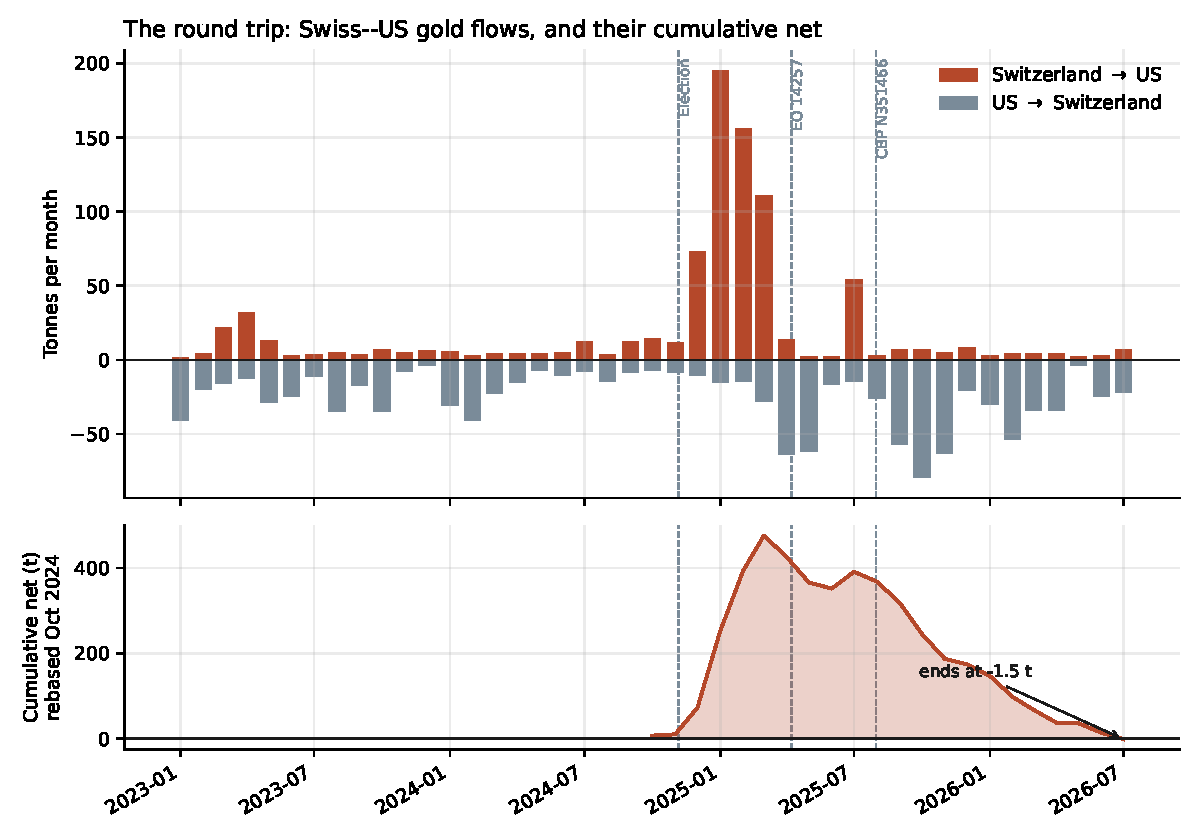
\includegraphics[width=\textwidth]{figures/fig1_roundtrip.pdf}
\caption{The round trip. Upper panel: monthly Swiss--US gold flows in both directions. Lower
panel: cumulative net, rebased to zero at October 2024. The cumulative line rises to roughly
$+476$ tonnes by March 2025 and returns to approximately zero by mid-2026. Source: BAZG
reported net mass.}
\label{fig:roundtrip}
\end{figure}

%==============================================================================
\section{The basis: measuring the price of relocation}
\label{sec:basis}
%==============================================================================

\subsection{Why the dollar spread is the wrong measure}

The signal that drives transatlantic gold relocation is the spread between the COMEX futures
price and the London spot price --- in practice quoted as an Exchange for Physical (EFP), a
privately negotiated swap of a COMEX futures position for an equivalent London OTC position.
Dealers quote the EFP as the price of relocating your exposure, which is precisely why it leads
physical relocation.

The true dealer EFP is not publicly available; it lives on entitlement-gated Bloomberg
contributor pages. What is constructible from public and purchased data is a synthetic
proxy: the COMEX settlement price minus the LBMA PM auction price. Throughout this
memorandum, ``basis'' means that proxy, and every quoted figure should be read with that
substitution in mind.

Reporting the basis in dollars per ounce, which is how it is almost always discussed, is
actively misleading across time for two reasons.

\textbf{First, it scales with the gold price.} A \$100 basis on \$4{,}400 gold and a \$58 basis
on \$2{,}790 gold are approximately the same proportional dislocation. Over the window studied
here the gold price rose from roughly \$2{,}650 to roughly \$4{,}480, so a dollar-denominated
basis series trends upward mechanically.

\textbf{Second, it scales with time to delivery.} A futures price embeds the cost of carrying
metal to delivery. That cost shrinks to zero as delivery approaches, so the dollar basis
exhibits a sawtooth driven purely by the contract calendar. At 4.5\% financing on \$4{,}400
gold, the pure-carry basis at sixty days is roughly \$33 and at zero days is zero. A \$33 swing
with no economic content whatsoever --- the same order of magnitude as the January 2025
dislocation.

The fix is to convert to an annualised implied financing rate and subtract the rate that carry
alone would justify:
\begin{align}
r^{\text{implied}}_t &= \left(\frac{F_t}{S_t} - 1\right)\cdot\frac{365}{d_t} \\[0.3em]
\text{dislocation}_t &= r^{\text{implied}}_t - \left(r^{\text{short}}_t + \sigma\right)
\end{align}
where $F_t$ is the COMEX settlement price of the most-active contract, $S_t$ the LBMA PM fix,
$d_t$ days to first notice, $r^{\text{short}}$ the overnight rate (SOFR from 3 April 2018,
effective fed funds before), and $\sigma$ an assumed all-in storage and insurance cost of
0.25\%/yr. The storage term is an assumption --- no free public series exists --- but it is
small relative to the dislocations discussed and does not affect any ranking.

Three construction choices deserve to be stated because they are not innocuous:

\begin{enumerate}[leftmargin=*]
\item \textbf{Settlement, not close.} CME's official daily settlement is not the last trade of
the session, and it is the number against which an EFP is struck. Using a closing price
introduces noise of a few dollars --- immaterial in 2020, material when the quantity of
interest is a \$10 excess basis.
\item \textbf{Most-active contract by open interest, not calendar front month.} The
calendar-nearest contract is frequently illiquid. Rolling on open interest reproduces what a
dealer would actually quote, and makes the roll date an output of the data rather than an
imposed convention.
\item \textbf{First notice, not last trade, as the horizon.} A holder must close or roll before
first notice to avoid delivery, so first notice is the economically binding date. It is
computed as the last weekday of the month preceding the contract month, ignoring exchange
holidays, which can shift it by a day or two.
\end{enumerate}

Observations within twenty days of first notice are dropped from all rate statistics. As $d_t
\to 0$ the annualisation factor $365/d_t$ explodes and a one-tick basis becomes a double-digit
``rate.'' The threshold is a judgement call; the ranking of episodes is unchanged at ten or
thirty days.

\subsection{The result, and the central puzzle}

\begin{table}[h]
\centering
\small
\begin{tabular}{@{}lrrrrr@{}}
\toprule
\textbf{Episode} & \textbf{Mean} & \textbf{Max} & \textbf{Max raw} & \textbf{Mean} &
\textbf{CHE$\to$US flow} \\
 & \textbf{disloc.} & \textbf{disloc.} & \textbf{basis} & \textbf{spot} & \textbf{(t/month)} \\
\midrule
Calm baseline, 2015--2019 & $-0.12\%$ & 27.0\% & \$33.80 & \$1{,}269 & 2.6 \\
COVID, Mar--May 2020 & \textbf{7.60\%} & 31.1\% & \$72.15 & \$1{,}666 & 94.7 \\
Tariff anticipation, Nov 2024 -- Apr 2025 & 1.16\% & 13.3\% & \$57.95 & \$2{,}796 &
\textbf{109.7} \\
Post-exemption, Apr--Jul 2025 & 0.23\% & 13.2\% & \$65.25 & \$3{,}308 & 19.6 \\
CBP bar ruling, Aug--Oct 2025 & 0.42\% & 9.8\% & \textbf{\$102.20} & \$3{,}707 & 5.4 \\
Unwind, Jan--Aug 2026 & $-0.77\%$ & 19.4\% & \$112.95 & \$4{,}590 & 4.0 \\
\bottomrule
\end{tabular}
\caption{Basis dislocation and physical flow by episode. Dislocation is the annualised excess
over carry; ``max raw basis'' is the largest single-day COMEX-minus-London spread in dollars.
Flow is Swiss-reported exports to the US, averaged per month within the window.}
\label{tab:puzzle}
\end{table}

Table~\ref{tab:puzzle} contains the memorandum's central empirical finding, and it is not the
finding I expected.

\textbf{Measured properly, the 2024--25 tariff episode was a much smaller financial dislocation
than March 2020} --- a mean excess of 1.16\% annualised against COVID's 7.60\%, roughly
one-seventh. And yet the physical flow was \emph{larger}: 109.7 tonnes per month against
COVID's 94.7, sustained over a longer window.

Normalising, the tariff episode moved roughly 95 tonnes per month per percentage point of
dislocation; COVID moved roughly 12. \textbf{The same price signal bought almost eight times
more metal in 2025 than in 2020.}

The August--October 2025 window makes the point even more sharply, and in the opposite
direction. Following the CBP ruling the raw dollar basis reached \$102.20 --- the widest of the
entire tariff era, and the number that generated most of the press coverage. The flow response
was 5.4 tonnes per month, essentially nothing.

The dollar spread and the flow are close to orthogonal. Any model that regresses tonnage on the
dollar basis is fitting the gold price and the delivery calendar.

\begin{figure}[htbp]
\centering
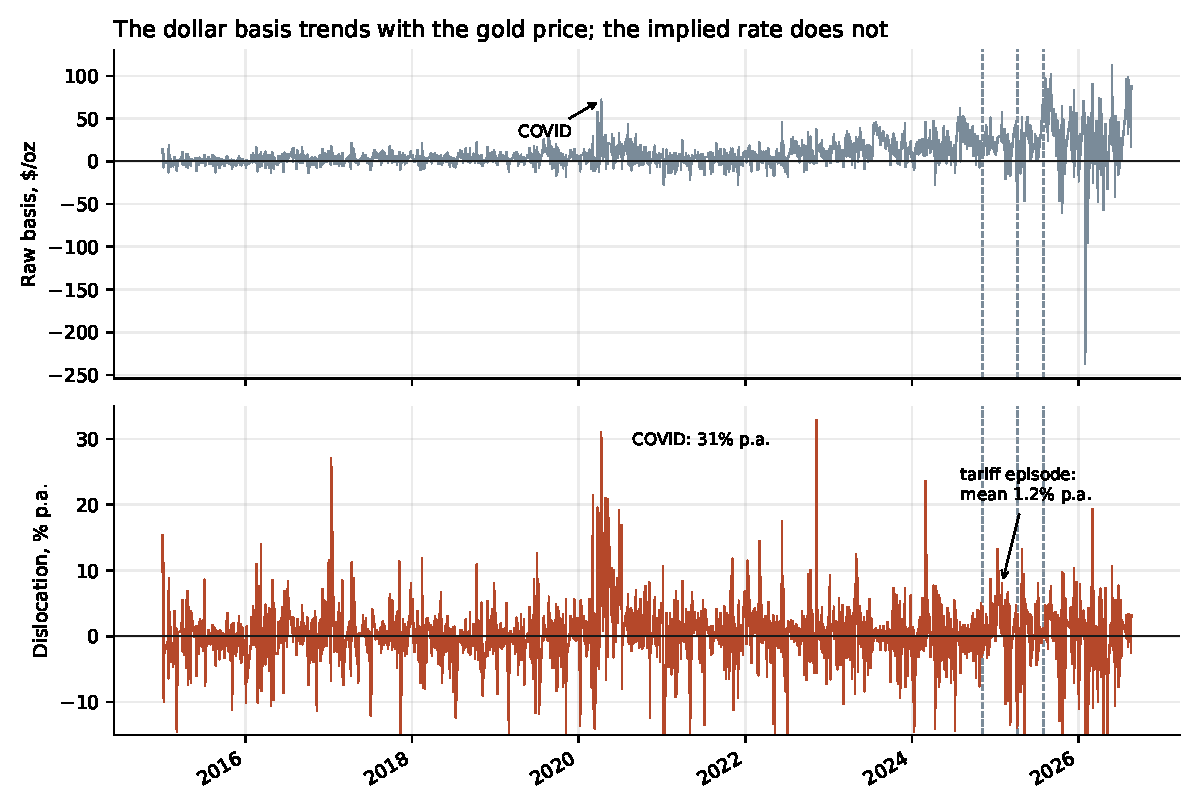
\includegraphics[width=\textwidth]{figures/fig2_basis.pdf}
\caption{Why the measure matters. The upper panel is the raw COMEX-minus-London dollar spread,
which drifts upward with the gold price and reaches its all-time highs in 2026. The lower panel
is the same data expressed as an annualised excess over carry, on which March 2020 dominates
everything else and the tariff episode is comparatively modest.}
\label{fig:basis}
\end{figure}

\subsection{Why: executability and expected persistence}

The resolution is that a basis dislocation is a \emph{price}, and the flow response depends on
two things the price does not contain: whether the arbitrage can physically be executed, and
whether it is expected to persist long enough to be worth executing.

\textbf{March 2020 was a dislocation caused by inability to move metal.} Swiss refineries in
Ticino shut under COVID restrictions; the great majority of bullion moves in the holds of
passenger aircraft, and passenger aviation stopped. The basis blew out to 7.6\% annualised
precisely \emph{because} arbitrageurs could not close it. High price, low executability,
moderate flow.

\textbf{November 2024 to April 2025 was a dislocation caused by a change in incentive with
logistics fully functional.} Refineries ran, freight ran, and the recast-and-fly cycle
completed in roughly a month. A modest but persistent basis was therefore enough to pull an
enormous quantity, because every tonne moved closed a little of the gap and the gap kept
reopening as the policy risk persisted. Moderate price, full executability, very large flow.

\textbf{August 2025 was a dislocation nobody expected to survive.} The CBP ruling produced a
very wide spread, but committing metal to a three-week shipping-and-recasting cycle only pays
if the spread is still there on arrival, and market participants evidently expected
clarification --- which arrived. Very high price, full executability, near-zero flow. By then,
in any case, the metal was already in New York; the trade had been done.

This generalises a warning that practitioners state narrowly: do not read the magnitude of a
spread as the intensity of a physical episode. The spread tells you what relocation is worth
per ounce at that instant. It tells you nothing about how many ounces will move, which depends
on physical capacity and on beliefs about duration.

\subsection{The basis does not lead the flow}

A claim this project previously carried --- and which appears in market commentary --- is that
the basis is a leading indicator of the following month's physical flow, with a lag of roughly
one month corresponding to the recast-and-fly cycle. The intuition is appealing and the
January 2025 episode appears to show it: the spread opened in December, the tonnage peaked in
January.

With eleven years of data the claim does not hold.

\begin{table}[h]
\centering
\begin{tabular}{@{}lrrrr@{}}
\toprule
\textbf{corr(dislocation$_{t-k}$, flow$_t$)} & $k=0$ & $k=1$ & $k=2$ & $k=3$ \\
\midrule
Full sample, $n=139$ & \textbf{$+0.55$} & $+0.51$ & $+0.35$ & $+0.20$ \\
Excluding COVID and tariff episodes, $n=125$ & $+0.27$ & $+0.17$ & $+0.17$ & $+0.19$ \\
\bottomrule
\end{tabular}
\caption{Cross-correlation of the monthly-average dislocation with Swiss$\to$US flow.}
\end{table}

The correlation is \emph{strongest contemporaneously} and decays monotonically with lag. A
one-month lead would show $k=1$ dominating; it does not.

Two honest qualifications. First, customs data is monthly, so this test cannot distinguish
``contemporaneous'' from ``leads by a few days or weeks'' --- a spread that opens on 10 December
and pulls metal that ships on 27 December appears contemporaneous at monthly frequency. The
result rules out a one-month lead, not a shorter one. Second, and more damaging to the general
claim: excluding the two crisis episodes, the correlation falls to $+0.27$ contemporaneously
and is essentially flat across lags. \textbf{The basis--flow relationship is a crisis-regime
phenomenon.} In ordinary months the spread carries little information about tonnage, which is
consistent with ordinary months' flow being dominated by genuine commercial demand rather than
arbitrage.

The earlier one-month-lead claim appears to have been inferred from roughly six observations
during a single episode. It is the kind of pattern that is very easy to see and very hard to
sustain.

\subsection{The response is kinked, and the threshold is near zero}

Arbitrage should not trigger until the basis exceeds the all-in cost of moving metal --- freight,
insurance, recasting, transit financing. Below that, nothing should move. The prediction is a
kinked response, not a linear one.

\begin{table}[h]
\centering
\begin{tabular}{@{}lrrrr@{}}
\toprule
\textbf{Monthly mean excess basis} & \textbf{Months} & \textbf{Mean flow (t)} &
\textbf{Median (t)} & \textbf{Max (t)} \\
\midrule
below $-\$5$ & 5 & 4.2 & 4.1 & 6.6 \\
$-\$5$ to \$0 & 56 & 4.8 & 2.2 & 25.6 \\
\$0 to \$5 & 63 & 12.3 & 4.1 & 155.8 \\
\$5 to \$10 & 8 & 27.7 & 11.1 & 85.5 \\
\$10 to \$20 & 6 & 73.4 & 54.2 & 195.4 \\
above \$20 & 1 & 112.4 & 112.4 & 112.4 \\
\bottomrule
\end{tabular}
\caption{Swiss$\to$US flow by excess-basis bin, 2015--2026. Note the flat floor of roughly
4--5 t/month whenever the excess basis is negative: this is the corridor's genuine commercial
throughput, independent of arbitrage.}
\label{tab:bins}
\end{table}

Fitting $\text{flow}_t = a + b\cdot\max(0,\; \text{excess}_t - c)$ over a grid of thresholds
gives a best fit at $c \approx \$0.5$/oz, with $b \approx 5.2$ tonnes per dollar per month.
The kinked specification explains $R^2 = 0.354$ against $0.232$ for a plain linear fit --- a 52\%
improvement --- confirming that the convexity is real and not an artefact of the two large
episodes.

\begin{figure}[htbp]
\centering
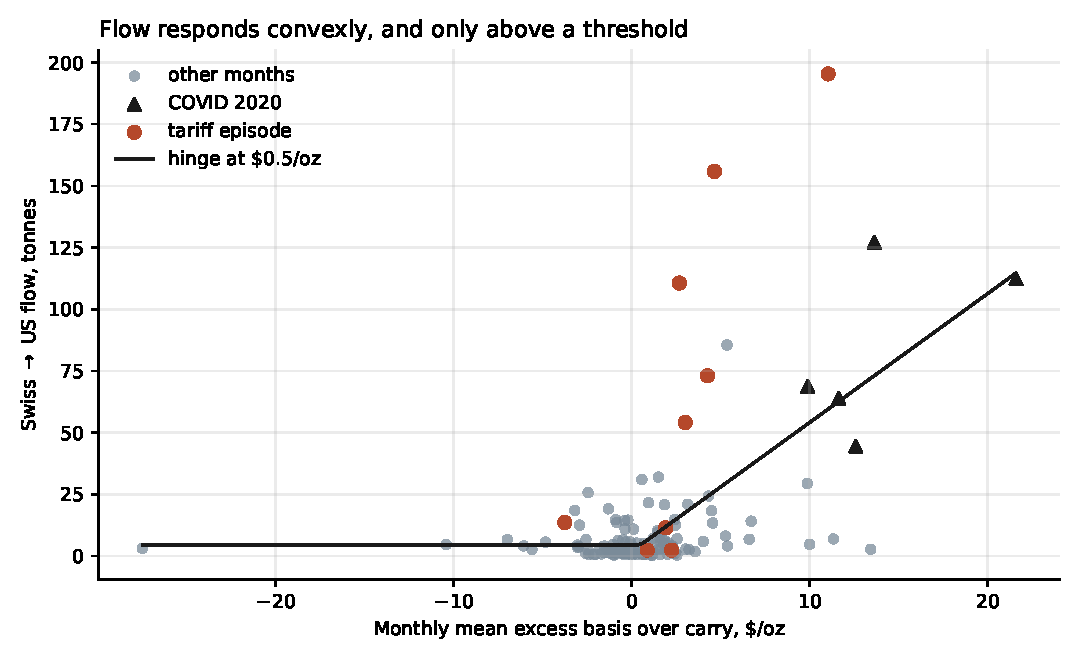
\includegraphics[width=0.92\textwidth]{figures/fig6_kink.pdf}
\caption{Monthly flow against monthly mean excess basis. Note that the tariff-episode
observations (filled circles) sit systematically \emph{above} the fitted hinge while the COVID
observations (triangles) sit on or below it --- the same ``more metal per unit of signal''
result as Table~\ref{tab:puzzle}, in a different projection.}
\label{fig:kink}
\end{figure}

The estimated threshold should be treated as indicative rather than as a measurement of
transatlantic transfer cost, for three reasons. It is fitted on monthly averages, which
attenuate the daily variation that actually drives shipping decisions. It is identified largely
off two episodes. And the flow series has a floor of genuine commercial trade around 4--5
tonnes per month that a two-parameter hinge cannot separate from a small arbitrage response.
A threshold of \$0.5/oz over carry is plausibly at the low end of quoted all-in transfer costs;
a daily-frequency version of this exercise, with a true dealer EFP, would be worth doing and is
noted in \S11.

\subsection{A note on the direction of the 2026 basis}

The 2026 mean dislocation is \emph{negative} ($-0.77\%$): COMEX has been persistently cheap
relative to London. That is the arbitrage running in reverse, and it is exactly what the flow
data shows --- 203.4 tonnes moving US$\to$Switzerland in seven months against 27.8 tonnes
moving the other way. The unwind is not a passive decay of the 2025 build; it is an actively
priced flow in the opposite direction.

%==============================================================================
\section{The classification discovery}
\label{sec:classification}
%==============================================================================

This section documents a finding that began as a suspected bug and turned out to be a
substantive result about the measurement of the episode.

\subsection{The anomaly}

Cross-checking the Swiss export series against the US import series --- the same physical
shipments, recorded by two authorities --- initially produced a catastrophic mismatch. For
January 2025 Switzerland reported 195.4 tonnes shipped to the United States. US Census data
for HS 7108, non-monetary gold, recorded \$0.57 billion of imports from Switzerland: at the
prevailing price, roughly 6.6 tonnes. A discrepancy of a factor of thirty.

The resolution is that the two authorities put the same metal in different chapters of the
tariff schedule.

\begin{table}[h]
\centering
\begin{tabular}{@{}lrrrr@{}}
\toprule
& \multicolumn{2}{c}{\textbf{Switzerland reports (t)}} &
  \multicolumn{2}{c}{\textbf{US reports (implied t)}} \\
\cmidrule(lr){2-3}\cmidrule(lr){4-5}
\textbf{Month} & \textbf{HS 7108} & \textbf{HS 7115} & \textbf{HS 7108} & \textbf{HS 7115} \\
\midrule
Oct 2024 & 14.3 & 0.0 & 1.3 & 10.0 \\
Nov 2024 & 11.4 & 0.0 & 1.5 & 12.2 \\
Dec 2024 & 73.1 & 0.0 & 14.5 & 73.6 \\
Jan 2025 & 195.3 & 0.1 & 6.6 & \textbf{217.0} \\
Feb 2025 & 155.8 & 0.0 & 1.1 & \textbf{172.1} \\
Mar 2025 & 110.5 & 0.0 & 0.2 & \textbf{111.4} \\
Apr 2025 & 13.6 & 0.0 & 1.2 & 10.4 \\
Jul 2025 & 54.1 & 0.0 & \textbf{54.0} & 2.6 \\
\bottomrule
\end{tabular}
\caption{The same shipments, two classifications. Swiss figures are reported net mass; US
figures are implied from customs value divided by the USGS monthly average gold price, so they
carry conversion error of roughly $\pm$10\%. Note that the \emph{totals} reconcile closely ---
Jan 195.4 vs 223.6, Feb 155.8 vs 173.2, Mar 110.5 vs 111.6 --- while the \emph{composition} is
almost exactly inverted.}
\label{tab:classification}
\end{table}

Switzerland books the episode as gold (HS 7108). The United States books it as ``articles of
precious metal, not elsewhere specified'' (HS 7115.90). At the ten-digit level the US flow
runs almost entirely through 7115.90.0530, which went from a baseline of roughly \$0.9 billion
per month in autumn 2024 to \$18.65 billion in January 2025 and back to \$0.03 billion by May.

This is the CBP doctrine of \S3.1 operating in the data: branded, stamped, cast bars are not
``unwrought,'' and until the 2025 ruling the settled practice --- established by the 2002
revocation and a run of rulings through 2017 --- placed them in 7115.90.05xx.

\subsection{The reclassification is datable}

The most striking feature of Table~\ref{tab:classification} is the July 2025 row, where the
composition flips. From December 2024 through April 2025 the US recorded the flow under
7115.90; in July 2025 it recorded \$4.84 billion under 7108.12.1013 (gold bullion) and
\$0.72 billion under 7108.12.1017, with 7115.90 falling to \$0.28 billion. From September 2025
onward, HTS 7108.13.5500 --- the precise line CBP specified in ruling N351466 --- begins
appearing in the data for the first time in the sample (\$0.34bn in September, \$0.24bn in
October, \$0.57bn in December).

The ruling is dated 31 July 2025. The ruling request letter it answers is dated 18 July 2025.
The reclassification is visible in the trade data in the same month, and the specific new line
appears within two months.

\begin{figure}[htbp]
\centering
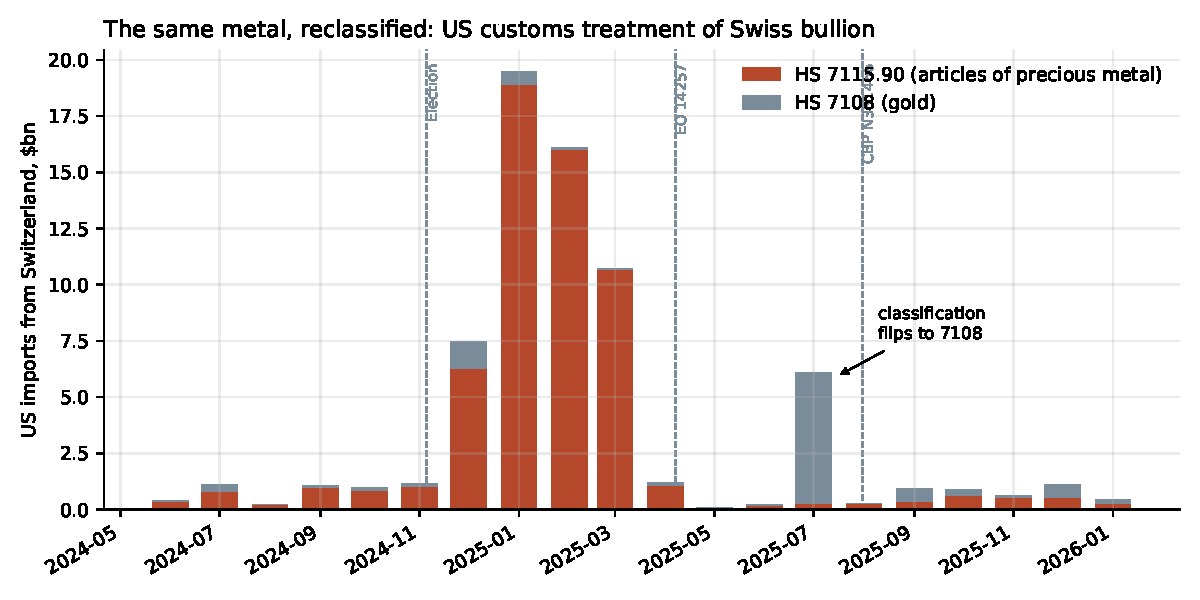
\includegraphics[width=\textwidth]{figures/fig5_classification.pdf}
\caption{US customs treatment of gold imported from Switzerland, by HS4 heading. The
December 2024 -- March 2025 episode is booked almost entirely under HS 7115.90; the July 2025
inflow is booked under HS 7108. The series ends January 2026, the limit of the Census extract
used here.}
\label{fig:classification}
\end{figure}

\subsection{Why this matters beyond bookkeeping}

Three consequences follow, and they are not small.

\textbf{The episode is invisible in several standard sources.} USGS's Monthly Mineral Industry
Survey publishes a US gold import table built from the gold-bearing-material headings --- ores,
doré, refined bullion, scrap. It reports total US gold imports from all countries of 43.0
tonnes in January 2025, in a month when Switzerland alone shipped 195.4 tonnes. USGS is not
wrong; it is measuring what it says it measures. But an analyst who takes USGS's gold trade
table as the US import series --- a completely reasonable thing to do --- will understate the
episode by roughly a factor of five, and will see no episode at all in the composition.

\textbf{Tariff exposure was a function of classification, which is why the ruling moved
markets.} The reciprocal tariff regime operates through Chapter 99 provisions attached to
specific HTS lines. Ruling N351466 attached 9903.01.25 to the standard COMEX delivery bars.
The question of which heading applied was therefore not a technicality; it \emph{was} the
question of whether the metal was dutiable. A market that watched the basis reach \$102 in the
weeks after the ruling was pricing a classification decision.

\textbf{Any HS-7108-only study of this episode is mis-specified.} This includes, by
construction, the Indian series used in this memorandum, whose commodity axis excludes HS 7115
with no available workaround. It is a real limitation, flagged again in \S\ref{sec:limits}.

\subsection{Three authorities, three classifications}

The US--Swiss divergence turns out not to be an isolated quirk. Extending the same mirror
comparison to the London--Zurich corridor --- the other leg of the arbitrage triangle, and one
that carries far more metal --- produces a parallel result.

\begin{table}[h]
\centering
\begin{tabular}{@{}lp{5.0cm}rr@{}}
\toprule
\textbf{Authority} & \textbf{Heading applied to bullion bars} & \multicolumn{2}{c}{\textbf{Full-sample mass (t)}} \\
\midrule
& & \textbf{7108.12} & \textbf{7108.13} \\
\cmidrule(l){3-4}
Switzerland (BAZG), exports to UK & 7108.12, unwrought & \textbf{2{,}491.3} & 81.6 \\
United Kingdom (HMRC), imports from CHE & 7108.13, semi-manufactured & 22.7 & \textbf{2{,}029.6} \\
\midrule
& & \textbf{7108} & \textbf{7115.90} \\
\cmidrule(l){3-4}
Switzerland, exports to US, Jan 2025 & 7108, gold & \textbf{195.3} & 0.1 \\
United States, imports from CHE, Jan 2025 & 7115.90, articles of precious metal &
6.6 & \textbf{217.0} \\
\bottomrule
\end{tabular}
\caption{The same physical product, classified three different ways. Swiss and UK figures are
reported net mass over the full 2015--2026 sample; US figures are implied tonnes for January
2025.}
\end{table}

Switzerland treats a cast, branded bullion bar as \emph{unwrought} gold. The United Kingdom
treats it as \emph{semi-manufactured}. The United States, until mid-2025, treated it as an
\emph{article of precious metal} --- not bullion at all in the chapter-71 sense --- and then, via
ruling N351466, moved to the UK's position.

The three positions are not arbitrary; they are three readings of the same rule. The
distinction between 7108.12 and 7108.13 turns on whether a bar has been ``processed otherwise
than by simple trimming.'' A cast bar stamped with a logo, weight, fineness, serial number and
QR code either has been or has not been, depending on how seriously one takes the stamping.
Switzerland says it has not; the UK says it has; the US said something stronger still.

Two implications follow for anyone building a gold trade panel.

First, \textbf{HS-code-level bilateral comparisons across these countries are not
apples-to-apples even when the aggregate mass reconciles}. Any study that filters on 7108.12,
or that treats 7108.12 and 7108.13 as economically distinct categories, will produce corridor
composition that is an artefact of which authority is reporting.

Second, and more consequentially: because tariff liability attaches to headings, and the three
authorities disagree about the heading, \textbf{the same bar's dutiable status was a function of
which border it was crossing and in which year}. That is not a measurement problem. It is a
statement about how the policy actually bit, and it is a large part of why a classification
ruling was capable of moving a basis by \$100 an ounce.

%==============================================================================
\section{Gross versus net: the phantom trade statistic}
%==============================================================================

\begin{table}[h]
\centering
\begin{tabular}{@{}lrr@{}}
\toprule
\textbf{Oct 2024 -- Jul 2026 (22 months)} & \textbf{Tonnes} & \textbf{USD bn} \\
\midrule
Switzerland $\to$ United States & 690.0 & 65.1 \\
United States $\to$ Switzerland & 691.5 & 82.3 \\
\midrule
\textbf{Gross recorded bilateral trade} & \textbf{1{,}381.5} & \textbf{147.4} \\
\textbf{Net change in position} & \textbf{$-1.5$} & \textbf{$-17.2$} \\
\midrule
Ratio, gross to $|$net$|$ (tonnes) & \multicolumn{2}{r}{$951\times$} \\
\bottomrule
\end{tabular}
\caption{The full round trip. Source: BAZG, reported net mass and BAZG's own USD conversion.}
\label{tab:grossnet}
\end{table}

Table~\ref{tab:grossnet} is the cleanest available statement of what the episode was.
Switzerland and the United States recorded 1{,}381.5 tonnes --- \$147.4 billion --- of gross
bilateral gold trade across twenty-two months, and finished with the United States holding
\emph{1.5 tonnes less} Swiss-origin gold than it started with. Some 1{,}382 tonnes of recorded
international commerce corresponded to approximately zero tonnes of net metal transfer.

The value column contains a second, subtler result that deserves separate attention. The metal
left the United States worth \$82.3 billion having arrived worth \$65.1 billion. The gold price
rose roughly 65\% over the window, so \textbf{the identical metal, returned to its origin,
registers as a \$17.2 billion bilateral goods deficit.} A trade balance measured in value can
therefore show a large and entirely spurious deficit arising from round-tripping inventory
during a price rally, with no net physical transfer and no economic transaction in any
meaningful sense.

This is not a hypothetical concern about statistical hygiene. Bilateral goods balances are
policy inputs. A tariff schedule calibrated on a deficit that includes non-monetary bullion in
transit is, to that extent, responding to vault geography and the gold price rather than to
commerce.

%==============================================================================
\section{Where the metal was: vaults}
\label{sec:comex}
%==============================================================================

\subsection{COMEX}

\begin{table}[h]
\centering
\begin{tabular}{@{}lrrrr@{}}
\toprule
\textbf{Date} & \textbf{Registered} & \textbf{Eligible} & \textbf{Pledged} & \textbf{Total} \\
\midrule
12 Nov 2019 & 34.9 & 224.2 & --- & 259.1 \\
3 Apr 2020 & 126.6 & 368.3 & --- & 494.9 \\
8 Oct 2020 & 544.0 & 618.5 & --- & 1{,}162.5 \\
7 Oct 2021 & 551.4 & 503.9 & --- & 1{,}055.3 \\
20 Apr 2023 & 382.6 & 307.3 & --- & 689.9 \\
\multicolumn{5}{c}{\emph{--- no archived snapshot for 21 months ---}} \\
30 Jan 2025 & 440.0 & 534.1 & 63.9 & 974.0 \\
28 Mar 2025 & 717.3 & 645.2 & 61.3 & 1{,}362.5 \\
\textbf{7 Apr 2025} & \textbf{752.3} & \textbf{645.9} & \textbf{62.2} & \textbf{1{,}398.2} \\
10 Jul 2025 & 628.4 & 514.5 & 68.4 & 1{,}143.0 \\
31 Dec 2025 & 602.2 & 530.0 & 61.0 & 1{,}132.3 \\
19 Aug 2026 & 451.5 & 378.4 & 53.3 & 829.9 \\
\bottomrule
\end{tabular}
\caption{COMEX gold warehouse stocks, tonnes, at observed snapshot dates. Recovered from
Internet Archive captures of CME's daily depository report.}
\label{tab:comex}
\end{table}

\textbf{A coverage limitation must be stated before any interpretation.} The archived record
contains no snapshot between 20 April 2023 and 30 January 2025. The pre-election COMEX level
therefore \emph{cannot be observed} in this dataset. Widely quoted figures for ``the build
since the election'' rest on a baseline this memorandum cannot verify, and no such figure is
quoted here. Every COMEX delta below runs between two observed dates.

\begin{table}[h]
\centering
\begin{tabular}{@{}lrrrr@{}}
\toprule
\textbf{Interval} & \textbf{Days} & \textbf{$\Delta$Total} & \textbf{$\Delta$Registered} &
\textbf{t/day} \\
\midrule
COVID build, Nov 2019 -- Oct 2020 & 331 & $+903.4$ & $+509.1$ & $+2.73$ \\
Tariff build, 30 Jan -- 7 Apr 2025 & 67 & $+424.2$ & $+312.3$ & \textbf{$+6.33$} \\
Drain, 7 Apr 2025 -- 19 Aug 2026 & 499 & $-568.3$ & $-300.8$ & $-1.14$ \\
\bottomrule
\end{tabular}
\caption{COMEX inventory changes between observed dates, tonnes.}
\end{table}

\begin{figure}[htbp]
\centering
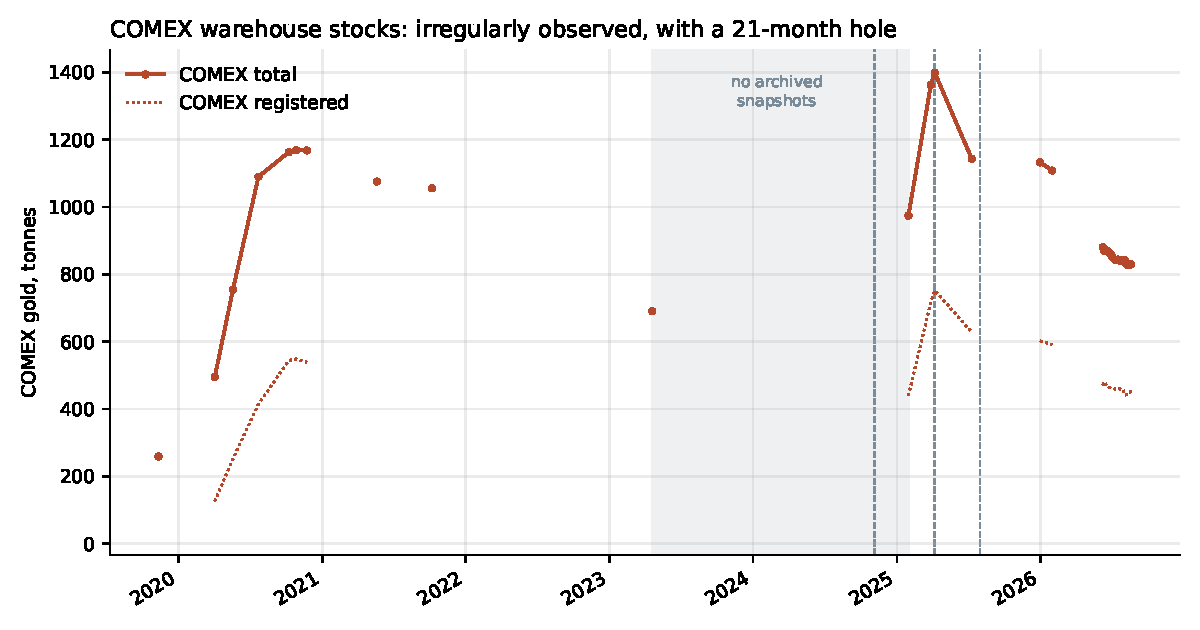
\includegraphics[width=\textwidth]{figures/fig3_comex.pdf}
\caption{COMEX warehouse stocks. Markers are observed snapshots; the line is broken wherever
consecutive observations are more than 120 days apart, so that gaps in the archival record
appear as gaps rather than as interpolated trends. The shaded region is the 21-month hole.}
\label{fig:comex}
\end{figure}

Three observations.

\textbf{The tariff build was faster than COVID's by a factor of 2.3 per day}, even though the
observable portion is smaller in total. This is consistent with the executability argument of
\S4.3: in 2020 the constraint was physical throughput, and the build took eleven months; in
2025 the logistics chain was unconstrained and the same order of magnitude arrived in ten
weeks.

\textbf{The build went disproportionately into registered stock} --- 74\% of the observed
increase. This matters because it rules out the most obvious artefact. COMEX inventory can rise
without any metal moving if metal already sitting in an approved depository as ``eligible'' is
re-warranted as ``registered.'' Here both categories rose, and the registered increase
(312.3 t) is substantially smaller than the Swiss inflow over an overlapping window, so the
build is not a reclassification illusion. Metal genuinely arrived and was genuinely warranted
for delivery.

\textbf{Metal leaves far more slowly than it arrives.} The drain ran at 1.14 t/day against the
build's 6.33 --- a factor of 5.6. Vault inventory is sticky in a way the price signal is not.

\subsection{London}

The dominant narrative in early 2025 held that New York's gain was London's loss, and that
London was being drained. The vault data does not support the strong form of this claim.

\begin{table}[h]
\centering
\begin{tabular}{@{}lrr@{}}
\toprule
\textbf{Month-end} & \textbf{London gold (t)} & \textbf{Change from Oct 2024} \\
\midrule
Oct 2024 & 8{,}775.3 & --- \\
Dec 2024 & 8{,}686.1 & $-89.2$ \\
Jan 2025 & 8{,}534.7 & $-240.6$ \\
\textbf{Feb 2025 (trough)} & \textbf{8{,}476.8} & \textbf{$-298.5$} \\
Mar 2025 & 8{,}488.4 & $-286.9$ \\
Jun 2025 & 8{,}775.6 & $+0.3$ \\
Dec 2025 & 9{,}106.4 & $+331.1$ \\
\textbf{Jul 2026} & \textbf{9{,}534.1} & \textbf{$+758.8$} \\
\bottomrule
\end{tabular}
\caption{LBMA London vault gold holdings, month-end. Includes ETF-allocated and Bank of England
metal.}
\end{table}

London's peak-to-trough drawdown was 298.5 tonnes, or \textbf{3.4\% of its holdings}. It was
fully recovered by June 2025 and London is now at a record 9{,}534 tonnes, 759 tonnes
\emph{above} its pre-episode level. Whatever happened in early 2025, ``London was drained'' is
not an accurate description of it.

\begin{figure}[htbp]
\centering
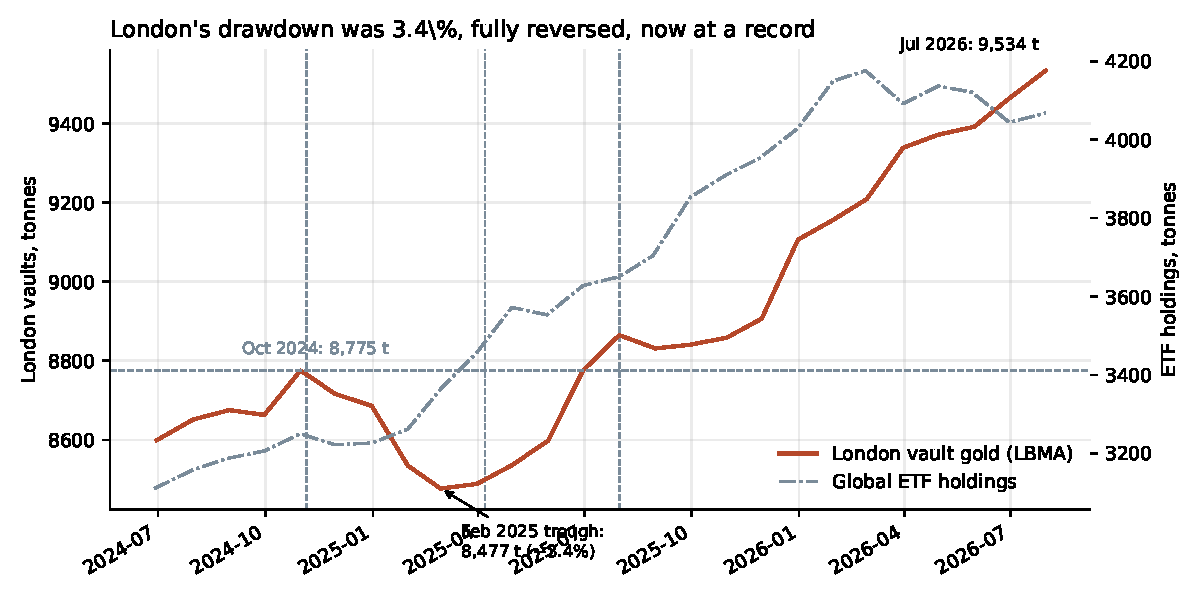
\includegraphics[width=\textwidth]{figures/fig4_london.pdf}
\caption{London vault gold (left axis) and global ETF holdings (right axis). The 2025 drawdown
is visible but shallow, and is followed by an uninterrupted climb to a record. ETF holdings rose
throughout, including during the drawdown.}
\label{fig:london}
\end{figure}

\subsection{Silver: the same experiment, run on a thinner market}
\label{sec:silver}

The LBMA publishes London silver vault holdings in the same workbook. Silver was subject to the
same tariff uncertainty --- it sits in the adjacent HS heading 7106 --- and trades in a market
with a much smaller float relative to its industrial offtake. If the 2025 episode was a genuine
London-to-New-York pull rather than a gold-specific accounting artefact, silver should show the
same signature, and it should show it more severely.

\begin{table}[h]
\centering
\begin{tabular}{@{}lrrrr@{}}
\toprule
\textbf{Month-end} & \textbf{Gold (t)} & \textbf{Index} & \textbf{Silver (t)} & \textbf{Index} \\
\midrule
Oct 2024 & 8{,}775.3 & 100.0 & 26{,}629.0 & 100.0 \\
Dec 2024 & 8{,}686.1 & 99.0 & 25{,}739.5 & 96.7 \\
Jan 2025 & 8{,}534.7 & 97.3 & 23{,}528.5 & 88.4 \\
Feb 2025 & 8{,}476.8 & \textbf{96.6} & 22{,}462.2 & 84.4 \\
Mar 2025 & 8{,}488.4 & 96.7 & 22{,}126.9 & \textbf{83.1} \\
Jun 2025 & 8{,}775.6 & 100.0 & 23{,}790.7 & 89.3 \\
Nov 2025 & 8{,}906.8 & 101.5 & 27{,}186.5 & 102.1 \\
Jul 2026 & 9{,}534.1 & 108.6 & 28{,}212.7 & 105.9 \\
\bottomrule
\end{tabular}
\caption{London vault holdings, indexed to October 2024 $=100$.}
\label{tab:silver}
\end{table}

It does, and it is not close. \textbf{Gold's London drawdown was 3.4\%; silver's was 16.9\%} ---
a fall of roughly 4{,}500 tonnes of silver, five times deeper in proportional terms. Silver also
took eight months longer to recover its starting level (November 2025 versus June 2025 for
gold).

This is a genuinely independent corroboration, and it is worth stating why. Nothing in the
silver series comes from the trade data, the COMEX data, or the basis construction; it is a
separate metal in a separate market, measured by the same vault operators. That it shows the
same shape, at a severity scaled to its thinner float, makes an accounting-artefact explanation
of the gold episode substantially harder to sustain.

A caution against over-reading it: this memorandum has no silver basis series, no silver lease
rates, and no silver trade data, so the mechanism is inferred by analogy rather than measured.
The claim is that the vault signature is consistent, not that the silver episode has been
analysed.

\subsection{Sourcing the build}

The drawdown is also too small to be the sole source of the COMEX build. Over a comparable
window, COMEX gained 424 tonnes at minimum while London lost 299. The Swiss corridor supplied
535 tonnes December to March. These figures do not net cleanly, which is expected: the flows
are asynchronous, the COMEX window is bounded by snapshot availability rather than by the
calendar, and the metal transiting Switzerland was not all of London origin.

One further consideration cuts against a simple London-to-New-York accounting. Global ETF
holdings \emph{rose} by 322 tonnes between October 2024 and April 2025, and ETF metal is
predominantly vaulted in London and included in the LBMA total. If ETF allocations grew by
roughly 322 tonnes while total London holdings fell by roughly 299, then non-ETF London
holdings --- closer to the concept of a free float --- fell by substantially more than the
headline. That decomposition is suggestive rather than exact, because WGC's ETF series is
global rather than London-only, and some funds vault in Zurich and New York. It is offered as
a caution about reading the headline vault number as the float, not as a measurement.

%==============================================================================
\section{Relocation or absorption? Five independent tests}
%==============================================================================

The claim that the episode was relocation rather than absorption is central, so it is worth
establishing from independent measurements rather than from a single decomposition.

\subsection{Test 1: the round trip}

The metal came back. Table~\ref{tab:grossnet}: net position change of $-1.5$ tonnes over
twenty-two months. Absorbed gold does not return to its origin.

\subsection{Test 2: the US re-export share}

US Census distinguishes \emph{domestic exports} (goods grown, produced or manufactured in the
United States) from \emph{re-exports} (foreign goods exported in the same condition as
imported). The re-export line is, by construction, an official measure of metal that entered
and left without being transformed or consumed --- relocation, as recorded by the exporting
government.

\begin{table}[h]
\centering
\begin{tabular}{@{}lrrr@{}}
\toprule
\textbf{Year} & \textbf{Domestic (\$bn)} & \textbf{Re-export (\$bn)} & \textbf{Re-export share} \\
\midrule
2015 & 12.40 & 0.04 & 0.3\% \\
2017 & 13.80 & 0.40 & 2.8\% \\
2019 & 14.45 & 0.50 & 3.4\% \\
2020 & 15.32 & 2.07 & 11.9\% \\
2022 & 20.83 & 8.58 & 29.2\% \\
2023 & 12.88 & 6.87 & 34.8\% \\
2024 & 16.99 & 5.39 & 24.1\% \\
\textbf{2025} & \textbf{47.63} & \textbf{34.88} & \textbf{42.3\%} \\
2026 (part) & 27.82 & 22.44 & 44.6\% \\
\bottomrule
\end{tabular}
\caption{US gold exports by type. In April 2025, the peak unwind month, the re-export share
reached 69\%.}
\label{tab:reexport}
\end{table}

In 2015--2019 essentially all US gold exports were domestic product; the re-export share
averaged under 3\%. In 2025 it was 42.3\%, and in the peak month 69\%. Nearly half of what the
United States now ``exports'' as gold is foreign metal passing through.

Table~\ref{tab:reexport} also contains a finding that is \emph{not} about tariffs, discussed
further in \S\ref{sec:trends}: the structural break is in 2022, not 2024.

\subsection{Test 3: the absorption bound}

Consumer absorption can now be measured directly rather than assumed. WGC reports quarterly
bar-and-coin and jewellery demand by country.

\begin{table}[h]
\centering
\begin{tabular}{@{}lrrrrr@{}}
\toprule
\textbf{Tonnes} & \textbf{Q4'24} & \textbf{Q1'25} & \textbf{Q2'25} & \textbf{Q3'25} &
\textbf{Q4'25} \\
\midrule
US bar and coin & 18.6 & 15.9 & 10.8 & 13.5 & 21.4 \\
US jewellery & 47.0 & 23.3 & 29.7 & 25.6 & 36.8 \\
\textbf{US consumer total} & \textbf{65.6} & \textbf{39.2} & \textbf{40.5} & \textbf{39.1} &
\textbf{58.2} \\
\bottomrule
\end{tabular}
\caption{US consumer gold demand, WGC. Note that this is an estimate produced by Metals Focus,
not a customs count.}
\end{table}

Total US consumer absorption in Q1 2025 was 39.2 tonnes, against an observed COMEX build of
424.2 tonnes over a slightly longer window. Even attributing the \emph{entire} quarter's US
jewellery and retail demand to the inflow --- which is indefensible, since jewellery
fabrication and 100\,oz COMEX warrants are different products drawn from different supply
chains --- absorption accounts for under 10\% of the build.

Notably, US retail bar and coin demand \emph{fell} during the episode, from 18.6 t in Q4 2024
to 10.8 t in Q2 2025. Whatever was arriving in New York, American households were not buying
it. This is the expected pattern for a price rally --- high prices suppress retail demand and
induce scrap --- and it is the opposite of what an absorption story requires.

\subsection{Test 4: corridor character}

If a corridor carries consumption, its flow should be relatively smooth and seasonal. If it
carries relocation, flow should be violently concentrated in episodes.

\begin{table}[h]
\centering
\begin{tabular}{@{}lrrrrr@{}}
\toprule
\textbf{Corridor} & \textbf{Mean (t)} & \textbf{CV} & \textbf{Max/median} &
\textbf{Top month} & \textbf{Top 6 months} \\
\midrule
CHE $\to$ United States & 13.2 & 2.19 & \textbf{48.5} & 10.6\% & \textbf{42.8\%} \\
CHE $\to$ United Kingdom & 15.6 & 1.52 & 21.8 & 5.2\% & 25.5\% \\
CHE $\to$ China & 26.0 & 0.82 & 7.0 & 4.4\% & 14.8\% \\
CHE $\to$ India & 26.4 & 0.71 & \textbf{3.8} & 2.3\% & \textbf{12.2\%} \\
\bottomrule
\end{tabular}
\caption{Swiss export corridors, monthly, 2015--2026, zero months excluded. ``Top 6 months''
is the share of all flow over the eleven-year sample concentrated in the six largest months.}
\label{tab:corridor}
\end{table}

The separation is stark. \textbf{The US corridor concentrates 42.8\% of eleven years of flow
into six months.} The India corridor concentrates 12.2\%, close to what one would expect from
seasonality alone (six months is 4.3\% of the sample, and Indian demand is strongly seasonal
around the festival and wedding calendar). The largest single month in the US corridor is 48.5
times the median month; in the India corridor, 3.8 times.

A methodological note, since it cost this project a false result earlier. The coefficient of
variation ranks these corridors correctly here, but it is a fragile statistic for this purpose:
near-zero months drag the mean down and compress the CV, so a relocation corridor with many
dormant months can score \emph{below} a consumption corridor. Max/median and concentration
shares are more robust and are reported alongside.

\subsection{Test 5: the inbound corridor was refining, not sourcing}

US gold imports during the build came almost exclusively from one country.

\begin{table}[h]
\centering
\begin{tabular}{@{}lrrrr@{}}
\toprule
\textbf{USD bn} & \textbf{Switzerland} & \textbf{United Kingdom} & \textbf{China} &
\textbf{India} \\
\midrule
Dec 2024 & 7.49 & 0.01 & 0.00 & 0.00 \\
Jan 2025 & 19.48 & 0.44 & 0.00 & 0.00 \\
Feb 2025 & 16.12 & 0.44 & 0.00 & 0.00 \\
Mar 2025 & 10.71 & 0.60 & 0.00 & 0.00 \\
\bottomrule
\end{tabular}
\caption{US gold imports by partner during the build.}
\end{table}

The United Kingdom --- the world's largest gold vaulting centre, and the presumed origin of
much of the metal --- shipped almost nothing directly. This is the transformation leg of the
taxonomy made visible: London holds 400\,oz Good Delivery bars, which are not deliverable
against a COMEX contract. The metal had to transit Switzerland to be recast into kilo and
100\,oz bars. London's inventory fell, but London's \emph{exports} to the US did not rise
correspondingly, because the metal was re-invoiced from Switzerland after recasting.

The outbound leg is different in character: during the unwind both Switzerland (\$0.59--11.53
bn/month) and the UK (\$0.40--4.51 bn/month) receive substantial volumes, because 100\,oz bars
returning to London do not necessarily require recasting to be stored, only to be Good Delivery.
This asymmetry --- in via one route, out via two --- is a concrete instance of why a single
correction factor for converting recorded trade into physical relocation cannot be right.

%==============================================================================
\section{What was actually happening underneath}
\label{sec:trends}
%==============================================================================

The premise of this exercise is that the phantom flows obscure genuine trends. Having removed
the noise, several such trends are visible, and they are largely unrelated to the tariff
episode.

\subsection{Chinese retail absorption rose sharply, and it was not about tariffs}

\begin{table}[h]
\centering
\begin{tabular}{@{}lrrrrrrr@{}}
\toprule
\textbf{Tonnes} & \textbf{Q4'24} & \textbf{Q1'25} & \textbf{Q2'25} & \textbf{Q3'25} &
\textbf{Q4'25} & \textbf{Q1'26} & \textbf{Q2'26} \\
\midrule
China bar and coin & 83.6 & 124.2 & 115.1 & 73.7 & 118.7 & \textbf{206.9} & 107.2 \\
China jewellery & 106.1 & 124.9 & 69.2 & 84.1 & 81.9 & 86.3 & 50.0 \\
India bar and coin & 76.0 & 46.7 & 46.1 & 91.6 & 96.0 & 62.3 & 50.3 \\
India jewellery & 189.8 & 81.6 & 88.8 & 125.0 & 145.3 & 66.1 & 75.1 \\
US bar and coin & 18.6 & 15.9 & 10.8 & 13.5 & 21.4 & 17.4 & 13.8 \\
\bottomrule
\end{tabular}
\caption{Consumer demand, WGC Gold Demand Trends, selected countries.}
\end{table}

Chinese bar and coin demand rose from 83.6 tonnes in Q4 2024 to 206.9 tonnes in Q1 2026 --- a
2.5-fold increase, and a level that dwarfs anything in the US series by an order of magnitude.
This is absorption in the strict sense: metal purchased by households and leaving the tradeable
float.

It is worth being precise about what this does and does not mean. Chinese retail demand rose
through a period in which the gold price also rose steeply, which is unusual --- retail demand
is normally price-elastic in the negative direction, as the Indian and US series show. Indian
jewellery demand collapsed from 189.8 t in Q4 2024 to 66.1 t in Q1 2026 as prices climbed;
US bar and coin demand fell. Chinese demand moved the other way. That divergence is
interesting and probably reflects domestic factors --- property market weakness, equity market
conditions, limited alternative savings vehicles --- but this memorandum has no data capable of
identifying the cause, and does not attempt to.

What can be said cleanly is that \textbf{the largest genuine absorption story of this period was
Chinese household demand, and it has no visible relationship to the transatlantic tariff
episode}. The two run on separate tracks, in different metal forms, through different corridors.

\subsection{Official sector accumulation: steady, and unrelated}
\label{sec:official}

The IMF's IRFCL series reports official reserve gold monthly in \emph{both} USD value and
millions of fine troy ounces. The distinction is critical. Over this window the gold price
roughly doubled, so the value of any unchanged holding rose dramatically; only the volume
series isolates actual accumulation.

\begin{table}[h]
\centering
\begin{tabular}{@{}lr@{\hskip 2em}lr@{}}
\toprule
\textbf{Month} & \textbf{$\Delta$ t} & \textbf{Month} & \textbf{$\Delta$ t} \\
\midrule
Jan 2024 & $+9.95$ & Jan 2025 & $+4.98$ \\
Feb 2024 & $+12.13$ & Mar 2025 & $+2.80$ \\
Mar 2024 & $+4.98$ & Jun 2025 & $+2.18$ \\
Apr 2024 & $+1.87$ & Sep 2025 & $+1.24$ \\
\textbf{May--Oct 2024} & \textbf{0.00 $\times$ 6} & Dec 2025 & $+0.93$ \\
Nov 2024 & $+4.98$ & Mar 2026 & $+4.98$ \\
Dec 2024 & $+10.26$ & Jun 2026 & $+14.93$ \\
\bottomrule
\end{tabular}
\caption{Monthly change in China's reported official gold holdings, tonnes, from IMF IRFCL
volume data. Level rose from 2{,}264.3 t (Oct 2024) to 2{,}346.4 t (Jun 2026).}
\end{table}

The pattern is worth describing precisely, and then not over-interpreting.

China reported \textbf{six consecutive months of zero change} (May--October 2024), then resumed
accumulation in November 2024 --- the month of the US election. Accumulation then
\emph{decelerated} steadily through 2025, falling to 0.93 t/month by late 2025, precisely as
the tariff drama was most intense. It re-accelerated sharply in 2026, reaching 14.93 t in June
2026.

Three quantitative statements can be made with confidence:

\begin{enumerate}[leftmargin=*]
\item Mean reported accumulation during the tariff-anticipation window was
\textbf{5.03 t/month}, against \textbf{5.22 t/month} outside it. There is no acceleration
associated with the episode.
\item The correlation between monthly reported accumulation and the monthly Switzerland-to-US
flow is \textbf{$r = -0.11$} (Pearson, $n=132$; Spearman $-0.11$). Statistically
indistinguishable from zero, and if anything faintly negative.
\item Total reported accumulation from November 2024 to June 2026 was \textbf{82.1 tonnes} over
twenty months --- against 690 tonnes moving Switzerland-to-US in a subset of that period. The
official-sector flow is roughly an order of magnitude smaller than the relocation flow.
\end{enumerate}

The honest conclusion is a negative one: \textbf{on the reported data, Chinese official
accumulation looks like a steady structural programme running on its own clock, unrelated to
the tariff episode.} The November 2024 resumption coincides in timing with the US election, and
it would be easy to build a narrative on that coincidence. It should be resisted. The
resumption is small (4.98 t), the programme decelerated through the period when the tariff
incentive was strongest, and the correlation with the actual relocation flow is zero.

\begin{figure}[htbp]
\centering
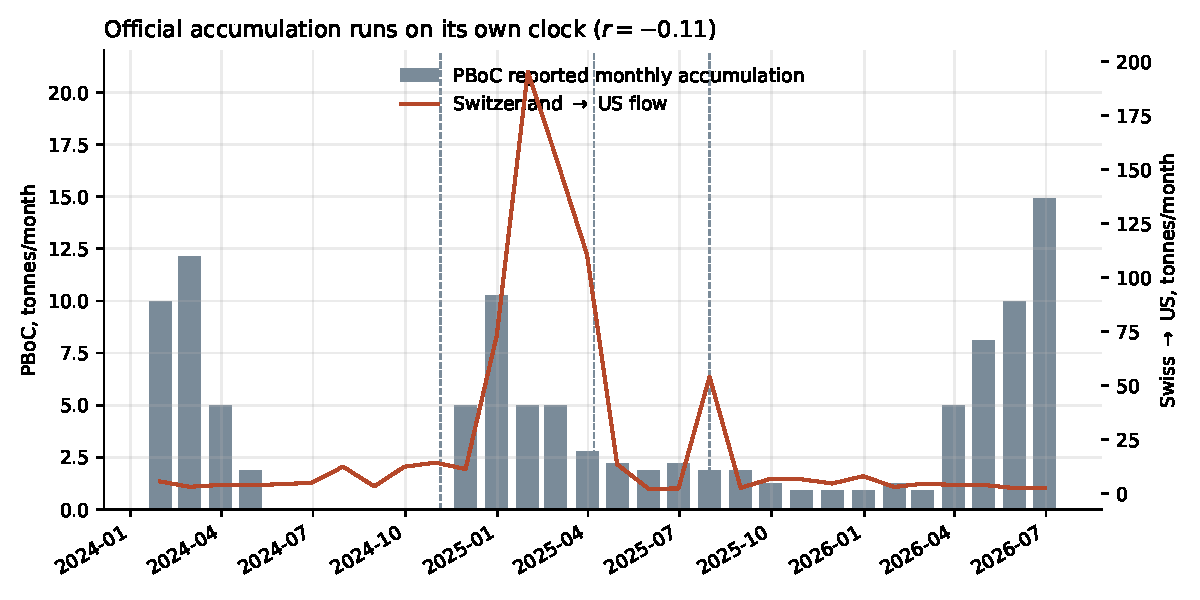
\includegraphics[width=\textwidth]{figures/fig7_pboc.pdf}
\caption{Reported Chinese official gold accumulation (bars, left axis) against the
Switzerland-to-US relocation flow (line, right axis). Note the six-month reporting pause ending
November 2024, the deceleration through 2025, and the re-acceleration in 2026. The two series
are on different scales by roughly an order of magnitude.}
\label{fig:pboc}
\end{figure}

Two caveats that cannot be resolved with these data. First, these are \emph{reported} figures,
and a substantial literature argues that Chinese official purchases exceed reported figures,
routed through channels that do not appear in IRFCL. This memorandum has no way to test that
and takes no position. Second, Shanghai Gold Exchange withdrawal data --- the standard
chokepoint measure for Chinese demand --- was not obtainable; the English-language SGE site
publishes only rendered HTML reports and the fuller series is Chinese-language. Any claim about
total Chinese absorption that relies on SGE is outside what is established here.

\subsection{The structural break is 2022, not 2024}

Table~\ref{tab:reexport} deserves a second look. The re-export share of US gold exports moved
as follows: under 3.5\% throughout 2015--2019; 11.9\% in 2020; 29.2\% in 2022; 34.8\% in 2023;
24.1\% in 2024; 42.3\% in 2025.

The tariff episode raised an already-elevated ratio. The regime change --- from a US gold export
business that was essentially all domestic product to one that is roughly a third to a half
transit metal --- happened in 2022, two years before any tariff was proposed.

This memorandum does not have the data to explain the 2022 break, and will not speculate beyond
noting that it coincides with the sanctioning of Russian gold and the associated re-routing of
global refined flows, and with the beginning of the Federal Reserve's hiking cycle, which
changed the economics of holding metal in any particular location. Both are plausible;
neither is tested here.

The methodological point stands independently: \textbf{an analyst who takes 2024 as the
pre-period and 2025 as the treatment period will attribute to tariffs a financialisation of US
gold trade that was already well underway.} The correct counterfactual is not 2024; it is
2019.

\subsection{ETFs accumulated throughout}

Global ETF holdings rose 322 tonnes between October 2024 and April 2025, and a further 496
tonnes from April 2025 to July 2026, reaching 4{,}068 tonnes. This is genuine investment
demand, it ran continuously through both the build and the unwind, and it is not a source for
COMEX registered stock --- ETF metal is held under a different custody arrangement and is
predominantly London-vaulted. If anything it competes with COMEX warrants for the same
underlying float.

The relevant point for this memorandum is that ETF accumulation provides an alternative
explanation for elevated gold demand throughout the period that has nothing to do with tariffs,
and that it did \emph{not} stop when the tariff arbitrage closed.

%==============================================================================
\section{Data quality: what the mirrors say}
%==============================================================================

Every bilateral flow in this study is, in principle, recorded twice --- once by the exporter and
once by the importer. Comparing the two is the cheapest available audit.

Across 1{,}457 corridor-months for which both sides report, only \textbf{63.4\%} fall within a
factor of two of each other. Disaggregated, the picture is much more informative than the
headline:

\begin{table}[h]
\centering
\begin{tabular}{@{}lrr@{}}
\toprule
\textbf{Corridor} & \textbf{Within 0.5--2$\times$} & \textbf{Median ratio} \\
\midrule
CHE $\to$ India & 98.6\% & 0.99 \\
CHE $\to$ United States & 97.0\% & 0.94 \\
CHE $\to$ United Kingdom & 84.8\% & 1.05 \\
GBR $\to$ Switzerland & 53.6\% & 1.01 \\
GBR $\to$ United States & 36.8\% & 1.03 \\
GBR $\to$ India & 22.4\% & 0.21 \\
IND $\to$ United States & 12.3\% & 0.00 \\
IND $\to$ United Kingdom & 2.6\% & --- \\
\bottomrule
\end{tabular}
\caption{Reporter/partner agreement by corridor.}
\end{table}

\textbf{Swiss-reported corridors are excellent} --- 85--99\% agreement, median ratios within a
few percent of unity. This is a strong endorsement of leaning on BAZG data, which this
memorandum does throughout.

\textbf{Indian-reported corridors are unusable at the monthly level}, but the reason is
mechanical rather than substantive. The TradeStat export interface reports in US\$ million
rounded to two decimals, so any flow under roughly \$5{,}000 in a month reports as literal zero
while the partner records a real positive value. The median ratio of exactly 0.00 for
India$\to$US is this artefact, not evidence of unreported trade.

\textbf{The GBR$\leftrightarrow$CHE monthly mismatch resolves into timing noise plus a third
classification convention.} At monthly frequency this corridor looks alarming: only 53.6\% of
GBR$\to$CHE months agree within a factor of two, and individual months are wild (December 2023:
Switzerland reports \$27.99m of imports from the UK against a UK-reported \$13{,}608 of exports
to Switzerland). The disagreement runs in both directions --- 42 months where the UK figure is
far larger, 22 where the Swiss figure is --- which already argues against systematic
under-reporting by either side.

At \emph{annual} frequency the corridor reconciles almost perfectly:

\begin{table}[h]
\centering
\small
\begin{tabular}{@{}lrrrrrrrr@{}}
\toprule
\textbf{CHE $\to$ GBR (t)} & \textbf{2019} & \textbf{2020} & \textbf{2021} & \textbf{2022} &
\textbf{2023} & \textbf{2024} & \textbf{2025} & \textbf{2026} \\
\midrule
UK says imported & 393.7 & 128.9 & 70.8 & 55.4 & 59.2 & 135.2 & 365.4 & 228.1 \\
Switzerland says exported & 385.7 & 132.6 & 78.7 & 55.0 & 74.5 & 151.6 & 390.6 & 265.7 \\
Ratio & 1.02 & 0.97 & 0.90 & 1.01 & 0.79 & 0.89 & 0.94 & 0.86 \\
\bottomrule
\end{tabular}
\caption{Annual agreement, CHE$\to$GBR corridor. Every year 2015--2026 falls between 0.79 and
1.02.}
\end{table}

The monthly disagreement is therefore shipment-timing --- consignments crossing a month boundary
differently on each side --- and not a level problem. This resolves a question this project had
previously left open as an unexplained anomaly.

The genuinely interesting residual is that the two authorities put the metal in different
subheadings. Over the full sample, of the metal the UK reports importing from Switzerland,
\textbf{2{,}029.6 tonnes is booked under HS 7108.13 (semi-manufactured) and only 22.7 tonnes
under 7108.12 (unwrought)}. Switzerland's mirror record of the same shipments is almost exactly
inverted: 2{,}491 tonnes under 7108.12 and 81.6 tonnes under 7108.13.

CEPII's BACI database, which produces one reconciled figure per exporter-importer-product-year,
sides with the \emph{importing} country in five of seven years in each direction for this
corridor. That is consistent with the standard presumption that import declarations are more
reliable than export declarations, since imports carry duty and scrutiny incentives that
exports do not. It is used in this project as a general reconciliation heuristic --- trust the
importer --- but it should be understood as validated on one corridor over seven years and
extrapolated elsewhere, not established.

%==============================================================================
\section{Limitations}
\label{sec:limits}
%==============================================================================

\begin{enumerate}[leftmargin=*]

\item \textbf{The COMEX baseline is unobserved.} No archived snapshot exists between April 2023
and January 2025. Any statement about the total build ``since the election'' is unavailable
here. This is the single most consequential gap, and it is a gap in the historical record as
recovered, not in the underlying data --- CME published the report daily throughout; it simply
was not archived and is not retrievable after the fact.

\item \textbf{The EFP is a proxy.} COMEX settlement minus LBMA PM is not a dealer EFP quote.
Its level can differ from a true EFP by the bid-offer and by any London forward basis. The
episode \emph{rankings} in Table~\ref{tab:puzzle} are robust to this; specific dollar figures
should be treated as indicative.

\item \textbf{Timestamp mismatch.} The LBMA PM auction fixes at 3pm London; COMEX settles at
1:30pm New York --- roughly ninety minutes apart. This is noise at monthly frequency but is not
noise on a day when the spread moved \$20 intraday. The single-day peak figures in this
memorandum carry that caveat.

\item \textbf{Storage cost is assumed, not measured.} The 0.25\%/yr figure is a convention. No
free public series exists. It shifts the dislocation level uniformly and affects no comparison.

\item \textbf{US tonnage is derived.} The Census pull has no quantity field, so any US-side
tonnage is value divided by an assumed monthly average price, carrying roughly $\pm$10\% error
in a period when the price moved 65\%.

\item \textbf{The Indian series excludes HS 7115.} TradeStat's commodity axis is a pre-defined
``GOLD'' bucket, confirmed by cross-reference against MEIDB's HS-code detail to comprise
7108.12/7108.13 plus incidental 7118.90 coin. Given \S\ref{sec:classification}, this is
potentially a serious omission, and it has no workaround within that data source.

\item \textbf{Re-warranting is invisible.} Metal already inside the United States that was
reclassified as COMEX-eligible generates no trade record and no public disclosure. This is the
asymmetry that defeats any single multiplier for converting recorded trade into physical
relocation, and it is unmeasurable with public data.

\item \textbf{Beneficial ownership is unavailable at any price.} LBMA and COMEX publish
location, never owner. The distinction between ``metal held in New York'' and ``metal owned by
Americans'' is unresolvable, not merely unresolved. Every claim in this memorandum is
territorial.

\item \textbf{WGC demand figures are estimates.} They originate with Metals Focus and inherit
that methodology. They are not customs counts and should not be treated as measurements of the
same kind as BAZG mass data.

\item \textbf{No SGE data.} Chinese domestic withdrawal data was not obtainable.

\item \textbf{Monetary gold is excluded by construction.} BPM6 excludes monetary gold from
merchandise trade, so central bank flows appear in none of the trade data used here; they enter
only via IRFCL and WGC reserves.

\end{enumerate}

%==============================================================================
\section{Replication}
\label{sec:replication}
%==============================================================================

This section is written so the analysis can be rebuilt without the code.

\subsection{Obtaining the data}

\begin{enumerate}[leftmargin=*]
\item \textbf{Swiss trade.} \texttt{opendata.swiss}, dataset ``Waren: Aussenhandel nach
Tarifnummer / Land.'' Two zipped CSVs (imports, exports), roughly 600\,MB each, all tariff
numbers and all partner countries, monthly from 2002. Filter to
\texttt{Tariffnumber4} $\in \{7108, 7115\}$, exclude \texttt{Tariffnumber6} $=$ 7115.10
(platinum catalysts), and to the partner countries of interest. Fields used:
\texttt{Quantity\_kg} and \texttt{Value\_USD}. \emph{Note the domain
\texttt{gate.bazg.admin.ch}, cited in older documentation, does not resolve.}

\item \textbf{US trade.} USA Trade Online, General Imports and Domestic/Foreign Exports, HTS
items, monthly, commodity list must include \textbf{both} 7108 and 711590. Registration
required. There is no quantity field in this export path.

\item \textbf{UK trade.} \texttt{api.uktradeinfo.com/OTS}, OData, no key. Filter on
\texttt{CommodityId} (71081100, 71081200, 71081310, 71081380, 71082000, 71159000, 71159010,
71159090) and \texttt{CountryId} (39 CHE, 400 USA, 664 IND, 720 CHN).
\texttt{FlowTypeId} 3 = non-EU imports, 4 = non-EU exports. Values are GBP.

\item \textbf{Indian trade.} \texttt{tradestat.commerce.gov.in/ftspcc/}, ``Commodity x Country
wise (Monthly).'' Commodity code \texttt{G6} = GOLD. Country codes 423 USA, 421 UK, 389 CHE,
77 CHN.

\item \textbf{COMEX stocks.} CME publishes \texttt{Gold\_Stocks.xls} at a fixed URL with no
historical archive. Historical values were recovered from Internet Archive captures via the CDX
API (\texttt{web.archive.org/cdx/search/cdx?url=cmegroup.com/delivery\_reports/Gold\_Stocks.xls}),
fetching each snapshot with the \texttt{id\_} raw modifier. Date each observation by the
report's own ``Activity Date'' field, not the crawl timestamp.

\item \textbf{COMEX futures.} Databento, dataset \texttt{GLBX.MDP3}, symbol \texttt{GC.FUT} with
\texttt{stype\_in=parent}. Two schemas: \texttt{ohlcv-1d} and \texttt{statistics}. In the
statistics schema, \texttt{stat\_type} 3 is settlement price and 9 is open interest.

\item \textbf{Prices and rates.} LBMA: \texttt{prices.lbma.org.uk/json/gold\_pm.json}, free, no
key, full history. Rates: FRED series \texttt{SOFR} (from April 2018), \texttt{DFF} before, and
\texttt{DEXUSUK} for GBP conversion.

\item \textbf{Vaults, demand, reserves.} LBMA London Vault Holdings workbook; WGC Goldhub
(registration) for Gold Demand Trends, ETF flows, and quarterly reserves; IMF IRFCL bulk CSV
for monthly reserve gold in both value and volume.

\item \textbf{Events.} Federal Register API (\texttt{federalregister.gov/api/v1}) --- note that
searching for ``gold'' fails, because the exemption is in a non-indexed annex; search the phrase
``reciprocal tariffs'' and select by date. CBP CROSS (\texttt{rulings.cbp.gov/api/search}),
free JSON, search term ``gold bar.''
\end{enumerate}

\subsection{Transformations applied}

\begin{enumerate}[leftmargin=*]
\item Convert all mass to tonnes at 32{,}150.7 troy oz/t. Convert GBP to USD at the
\texttt{DEXUSUK} monthly average.
\item Where a source reports only value, derive tonnage as value $\div$ (monthly average price
$\times$ 32{,}150.7) and label it implied.
\item Aggregate HTS/CN8 codes to HS4 by taking the first four characters of the code
\emph{as reported}. Do not zero-pad first: a six-digit code left-padded to ten digits yields a
spurious HS4 of ``0000.''
\item For the futures series: keep only outright contracts (exclude spread symbols such as
\texttt{GCJ5-GCV5}, which carry negative prices); parse the contract month from the symbol;
compute first notice as the last weekday of the preceding month; on each date select the
contract with the highest open interest among those still ahead of first notice.
\item Compute the implied rate and dislocation per equations (1)--(2). Drop observations with
fewer than twenty days to first notice before computing any rate statistic.
\item For COMEX stocks, never interpolate between snapshots. Report deltas between observed
dates only.
\item For the LBMA workbook, note that the most recent row's month label is blank; assign it
from the file title.
\item For IMF IRFCL, use the volume series (millions of fine troy ounces), not the value
series. The bulk export repeats each country-indicator across several internal series codes;
de-duplicate by keeping the series with the most observations.
\end{enumerate}

\subsection{Reproducing the headline figures}

\begin{itemize}[leftmargin=*]
\item \textbf{1{,}381.5 t gross, $-1.5$ t net}: sum BAZG Swiss-reported exports to and imports
from the US, HS 7108 + 7115, October 2024 through July 2026 inclusive, using reported net mass.
\item \textbf{1.16\% vs 7.60\% dislocation}: mean of the dislocation series over
5 Nov 2024 -- 6 Apr 2025 and 1 Mar -- 31 May 2020 respectively, after the twenty-day filter.
\item \textbf{424.2 t COMEX build}: difference in combined total between the 30 January 2025 and
7 April 2025 snapshots.
\item \textbf{298.5 t London drawdown}: LBMA month-end October 2024 minus February 2025.
\item \textbf{42.3\% re-export share}: US Census foreign exports $\div$ (domestic $+$ foreign
exports), HS 7108 $+$ 7115, calendar 2025, by value.
\item \textbf{42.8\% corridor concentration}: sum of the six largest monthly Swiss export
observations to the US, 2015--2026, divided by the sum of all non-zero months.
\item \textbf{16.9\% silver drawdown}: LBMA month-end silver, October 2024 minus March 2025,
from column three of the same workbook.
\item \textbf{Lead-lag correlations}: resample the daily dislocation to monthly means, join to
the monthly Swiss flow on month-end, and compute $\mathrm{corr}(\text{disloc}_{t-k},
\text{flow}_t)$ for $k=0\ldots3$. Repeat excluding March--August 2020 and November
2024--August 2025.
\item \textbf{Hinge threshold}: grid-search $c$ over $[-5, 20]$ in \$0.5 steps, fitting
$\text{flow}_t = a + b\max(0, \text{excess}_t - c)$ by OLS at each $c$ and selecting the
minimum residual sum of squares.
\end{itemize}

%==============================================================================
\section{What would settle the open questions}
%==============================================================================

Four things would materially improve on this, in descending order of value per unit of effort.

\textbf{A commercial COMEX warehouse stock series.} The twenty-one month archival gap is the
binding constraint on the central quantitative claim. Nick Laird's goldchartsrus, at roughly
\$180/yr, is reported to hold normalised daily series of exactly this kind; CME DataMine sells
the official history. Either would remove the largest caveat in this memorandum.

\textbf{A true dealer EFP series.} Bloomberg contributed pages, via
\texttt{BDH} on a contributor ticker. This would convert the basis analysis from indicative to
precise and would allow the kink --- the all-in transfer cost below which no arbitrage triggers
--- to be estimated rather than asserted. The value of that threshold is itself publishable:
transatlantic gold transfer cost has not been cleanly estimated in the literature.

\textbf{UK exports of HS 7108.13 to all destinations.} If the UK is genuinely shipping the mass
its own statistics claim, the ``missing'' metal in the GBR$\leftrightarrow$CHE mismatch may be
attributed to a different partner country in UK data. This is directly testable against the
same HMRC API already used, costs nothing, and would resolve whether the discrepancy is an
attribution problem or a genuine reporting gap.

\textbf{Shanghai Gold Exchange withdrawals.} Required for any serious statement about total
Chinese absorption as distinct from reported official reserves. Chinese-language source.

\vspace{1em}
\hrule
\vspace{0.5em}

\small
\noindent\textbf{A closing note on framing.} The instinct when confronted with 1{,}382 tonnes of
recorded trade and zero tonnes of net transfer is to call the trade fake. That is not quite
right, and the distinction matters for how one writes about it. The shipments were real,
insured, flown, recast, and warranted; freight forwarders and refiners were genuinely paid;
the arbitrage was genuinely profitable to whoever executed it. What is illusory is not the
activity but the \emph{inference} normally drawn from it --- that a bilateral goods flow of this
size reflects a change in what the two economies produce, consume, or owe each other. The gold
moved because its address was worth changing, and then the reason evaporated and it moved back.
Trade statistics faithfully recorded a real economic event; they simply do not record the event
most readers assume they are reading about.

\end{document}
